
% This LaTeX was auto-generated from MATLAB code.
% To make changes, update the MATLAB code and republish this document.











    
    \begin{DoxyCode}
function example_adjoint()
\end{DoxyCode}
\begin{par}
COMPILATION
\end{par} \vspace{1em}
\begin{DoxyCode}
    [exdir,~,~]=fileparts(which('example_adjoint.m'));
    % compile the model
    amiwrap('model_adjoint','model_adjoint_syms',exdir)
\end{DoxyCode}

         \begin{DoxyCode}Generating model struct ...
Parsing model struct ...

Generating C code ...
headers | wrapfunctions | 
Compiling mex file ...
amici | Building with 'Xcode with Clang'.
MEX completed successfully.
Building with 'Xcode with Clang'.
MEX completed successfully.
\end{DoxyCode} 
    \begin{par}
SIMULATION
\end{par} \vspace{1em}
\begin{DoxyCode}
    % time vector
    t = [linspace(0,4,5)];
    p = [1.1,0.3,1];
    k = [];

    D.Y = [     1.0171
        1.3423
        1.6585
        0.9814
        0.3288];

    D.Sigma_Y = 0.1*ones(size(D.Y));


    options.sensi = 1;
    options.sensi_meth = 'adjoint';
    options.maxsteps = 1e4;
    options.rtol = 1e-12;
    options.atol = 1e-12;
    % load mex into memory
    [~] = which('simulate_model_adjoint'); % fix for inaccessability problems
    sol = simulate_model_adjoint(t,log10(p),k,D,options);
\end{DoxyCode}
\begin{par}
Plot
\end{par} \vspace{1em}
\begin{DoxyCode}
    figure
    subplot(3,1,1)
    errorbar(t,D.Y,D.Sigma_Y)
    hold on
    % plot(t,sol.y)

    xlabel('time t')
    ylabel('observable')
    title(['log-likelihood: ' num2str(sol.llh) ])

    y = (p(2)*t + p(3)).*(t<2) + ( (2*p(2)+p(3)-p(2)/p(1))*exp(-p(1)*(t-2))+p(2)/p(1) ).*(t>=2);


    tfine = linspace(0,4,100001);
    xfine = (p(2)*tfine + 1).*(tfine<2) + ( (2*p(2)+p(3)-p(2)/p(1))*exp(-p(1)*(tfine-2))+p(2)/p(1) ).*(tfine>=2);

    mu = zeros(1,length(tfine));
    for it = 1:length(t)
        if(t(it)<=2)
            mu = mu + ((y(it)-D.Y(it))/(D.Sigma_Y(it)^2))*(tfine<=t(it));
        else
            mu = mu + ((y(it)-D.Y(it))/(D.Sigma_Y(it)^2))*exp(p(1)*(tfine-t(it))).*(tfine<=t(it)).*(tfine>2) + ((y(it)-D.Y(it))/(D.Sigma_Y(it)^2))*exp(p(1)*(2-t(it))).*(tfine<t(it)).*(tfine<=2);
        end
    end
    plot(tfine,xfine)
    legend('data','simulation')
    xlim([min(t)-0.5,max(t)+0.5])
    subplot(3,1,2)
    plot(tfine,mu)
    ylabel('adjoint')
    xlabel('time t')
    xlim([min(t)-0.5,max(t)+0.5])

    subplot(3,1,3)

    plot(fliplr(tfine),-cumsum(fliplr(-mu.*xfine.*(tfine>2)))*p(1)*log(10)*(t(end)/numel(tfine)))
    hold on
    plot(fliplr(tfine),-cumsum(fliplr(mu))*p(2)*log(10)*(t(end)/numel(tfine)))
    plot(tfine,-mu(1)*p(3)*log(10)*(tfine<2))
    xlim([min(t)-0.5,max(t)+0.5])
    ylabel('integral')
    xlabel('time t')

    legend('p1','p2','p3')

    grad(1,1) = -trapz(tfine,-mu.*xfine.*(tfine>2))*p(1)*log(10);
    grad(2,1) = -trapz(tfine,mu)*p(2)*log(10);
    grad(3,1) = -mu(1)*p(3)*log(10);

    plot(zeros(3,1),grad,'ko')
\end{DoxyCode}

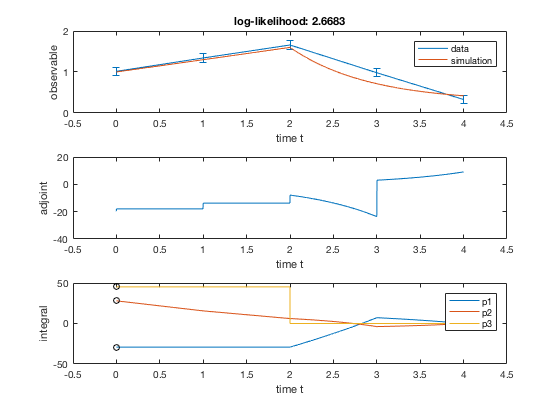
\includegraphics[width=\textwidth]{../../examples/example_adjoint/html/example_adjoint_01.png}
\begin{par}
FD
\end{par} \vspace{1em}
\begin{DoxyCode}
    eps = 1e-5;
    xi = log10(p);
    grad_fd_f = NaN(3,1);
    grad_fd_b = NaN(3,1);
    for ip = 1:3;
        options.sensi = 0;
        xip = xi;
        xip(ip) = xip(ip) + eps;
        solp = simulate_model_adjoint(t,xip,k,D,options);
        grad_fd_f(ip,1) = (solp.llh-sol.llh)/eps;
        xip = xi;
        xip(ip) = xip(ip) - eps;
        solp = simulate_model_adjoint(t,xip,k,D,options);
        grad_fd_b(ip,1) = -(solp.llh-sol.llh)/eps;
    end

    figure
    plot(abs(grad),abs(grad_fd_f),'o')
    hold on
    plot(abs(grad),abs(grad_fd_b),'o')
    plot(abs(grad),mean([abs(grad_fd_b),abs(grad_fd_f)],2),'o')
    plot(abs(grad),abs(sol.sllh),'o')
    plot([1e1,1e2],[1e1,1e2],'k:')
    set(gca,'XScale','log')
    set(gca,'YScale','log')
    axis square
    legend('forward FD','backward FD','central FD','adjoint sensintivity analysis','Location','SouthEast')
    xlabel('analytic absolute value of gradient element')
    ylabel('computed absolute value of gradient element')
    set(gcf,'Position',[100 300 1200 500])

    drawnow
\end{DoxyCode}

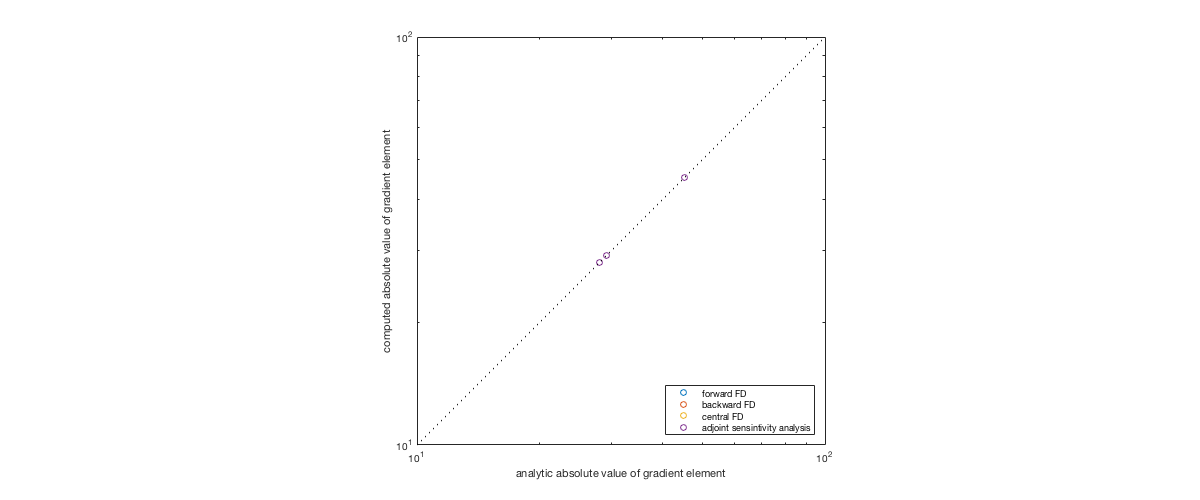
\includegraphics[width=\textwidth]{../../examples/example_adjoint/html/example_adjoint_02.png}
\begin{DoxyCode}
end
\end{DoxyCode}




    